
\chapter{Implementation}
This chapter focuses on the implementation of the elements described in the previous chapter.

\section{SQUISH-E Implementation}


\subsection{Algorithm 1}

\begin{lstlisting}[language=C, % Spécifie le langage du code
caption={SQUISH-E}, % Légende du listing
label=lst:squish_c, % Étiquette pour référencer le listing
numbers=left,
numberstyle=\tiny\color{gray},
stepnumber=1,
frame=single,
breaklines=true,
postbreak=\mbox{\textcolor{red}{$\hookrightarrow$}\space},
showstringspaces=false
]

void
iteration_simplification_sqe(void *p_i , void *p_j ,
size_t *beta,const double lambda,int i,
Dict *succ,Dict *pred,
PDict  *p,struct PriorityQueue *Q,
bool syncdist,interpType interp ,bool hasz ,uint32_t minpts)
{
if( i * lambda >= *beta)
{
*beta += 1;
}
set_priority_queue(p_i,INF,Q);
set_priority_dict(p_i,0,p);
if(i >= 1)
{
set_point_dict(p_i,p_j,pred);
set_point_dict(p_j,p_i,succ);
adjust_priority(p_j,Q,pred,succ,p, syncdist, interp , hasz );
}
size_t size = size_queue(Q);
if(size - *beta == 0 ){
reduce(Q,pred,succ,p,syncdist, interp , hasz );
}
}
\end{lstlisting}
\vspace{1cm}
This algorithm follow the pseudo code of SQUISH-E it called the set function of the priority queue and the set function of the point map and priority map that will be describe in the section about implementation of variable. Then the reduce function and adjust priority is called in order to reduce if the size meet the treshold and the adjustment for each point that has a predecessor and a successor in order to know the error that it will produce by removing the corresponding point.

\subsection{Algorithm 2}
\begin{lstlisting}[language=C, % Spécifie le langage du code
caption={reduce}, % Légende du listing
label=lst:reduce_c, % Étiquette pour référencer le listing
numbers=left,
numberstyle=\tiny\color{gray},
stepnumber=1,
frame=single,
breaklines=true,
postbreak=\mbox{\textcolor{red}{$\hookrightarrow$}\space},
showstringspaces=false
]

void
reduce(struct PriorityQueue *Q,Dict *pred,Dict *succ,PDict  *p,
bool syncdist,interpType interp ,bool hasz )
{
struct PriorityQueueElem *entry = remove_min(Q);
size_t size_before = size_queue(Q);

void * p_j = entry->point;
double priority = entry->priority;

void * p_i = get_point_dict(p_j,pred);
void * p_k = get_point_dict(p_j,succ);

double pr_i = get_priority_dict(p_i,p); if(priority > pr_i){ pr_i = priority; }
double pr_k = get_priority_dict(p_k,p); if(priority > pr_k){ pr_k = priority; }

set_priority_dict(p_k, pr_k ,p);
set_priority_dict(p_i, pr_i ,p);

set_point_dict(p_i,p_k,succ);
set_point_dict(p_k,p_i,pred);
set_point_dict(p_k,p_i,pred);

adjust_priority(p_k ,Q,pred,succ,p,syncdist, interp ,hasz );
adjust_priority(p_i ,Q,pred,succ,p,syncdist, interp ,hasz );


//Delete pointer
free(entry);
destroy_elem_PriorityDict(p_j,p);
destroy_elem_PointDict(p_j,succ);
destroy_elem_PointDict(p_j,pred);

}

\end{lstlisting}

This algorithm describe the reduction method as mentioned above remove the lowest priority points from the queue and it update the neighbors. Because we use C langage we free memory of the useless data.

\subsection{Algorithm 3}

\begin{lstlisting}[language=C, % Spécifie le langage du code
caption={adjust\_priority}, % Légende du listing
label=lst:adjust_c, % Étiquette pour référencer le listing
numbers=left,
numberstyle=\tiny\color{gray},
stepnumber=1,
frame=single,
breaklines=true,
postbreak=\mbox{\textcolor{red}{$\hookrightarrow$}\space},
showstringspaces=false
]

void
adjust_priority(void *p_i,struct PriorityQueue *Q, Dict *pred,Dict *succ,PDict  *p,
bool syncdist,interpType interp ,bool hasz )
{

void * p_h = get_point_dict(p_i,pred);
void * p_k = get_point_dict(p_i,succ);
if( p_h != NULL &&  p_k != NULL )
{
if(syncdist)
{
double priority = get_priority_dict(p_i,p) + SED(p_h,p_i,p_k, interp , hasz );
set_priority_queue(p_i,priority,Q);
}
}
}

\end{lstlisting}

\section{Variables Implementation}
In this section we'll discuss how the variables have been implemented and how effective they are, followed by a discussion of the performance and complexity achieved.

\subsection{Map}
In this section we will focus on the implementation of the map

\begin{lstlisting}[language=C, % Spécifie le langage du code
caption={Map C implementation}, % Légende du listing
label=lst:map_c, % Étiquette pour référencer le listing
numbers=left,
numberstyle=\tiny\color{gray},
stepnumber=1,
frame=single,
breaklines=true,
postbreak=\mbox{\textcolor{red}{$\hookrightarrow$}\space},
showstringspaces=false
]

#include <search.h>


typedef struct PriorityDict
{
void * key;
double priority;
} PriorityDict;


typedef struct PointDict
{
void *key;
void *value;
} PointDict;


typedef void* Dict;
typedef void* PDict;

\end{lstlisting}
\vspace{1cm}
This structure is a Map that link a point to a corresponding value like priority or another point. We just need to define a struct with two values the key and the value. The typedef void* is using for the GNU Library to avoid using void** and add more clarity to the code.

\paragraph{Method}

\begin{lstlisting}[language=C, % Spécifie le langage du code
caption={Point Map Methods}, % Légende du listing
label=lst:pmap_c, % Étiquette pour référencer le listing
numbers=left,
numberstyle=\tiny\color{gray},
stepnumber=1,
frame=single,
breaklines=true,
postbreak=\mbox{\textcolor{red}{$\hookrightarrow$}\space},
showstringspaces=false
]

void *
get_point_dict(void *p_i,Dict *dict)
{
PointDict find;
find.key = p_i;
void * result = tfind(&find, dict, compar);
if(result){
result = (*(PointDict**)result)->value;
}
return result;
}


void
set_point_dict(void * p_i,void * p_j,Dict *dict)
{
PointDict *find = malloc(sizeof(PointDict));
find->key = p_i;
find->value = p_j;
void * result = tfind(find, dict, compar);
if(result){
(*(PointDict**)result)->value = p_j;
}
else{
tsearch(find, dict, compar); /* insert */
}
}


void destroy_elem_PointDict(void * p_i,Dict *dict)
{
PointDict find;
find.key = p_i;
void * r = tfind(&find, dict, compar);
if(r)
{
PointDict * to_free = (*(PointDict**)r);
tdelete(&find,dict,compar);
free(to_free);
}
}

\end{lstlisting}

\vspace{1cm}
Here we use function of GNU C Library that implement a binary tree. It has the property to have for each operation a maximal complexity of $O(log(n))$ The two mapping use the same implementation in reality it would be a good idea to resolve this duplication case using a template or thing that can resolve it but the C language limit the capability.

\paragraph{Discussion}
As mentioned in the previous sub section the map use GNU C Library binary tree structure to perform search and set. Those algorithm have a complexity of $O(log(n))$ as mentioned before and it has the property to be have a dynamic allocation of memory.

\subsection{PriorityQueue}

\begin{lstlisting}[language=C, % Spécifie le langage du code
caption={PriorityQueue}, % Légende du listing
label=lst:prqueue_c, % Étiquette pour référencer le listing
numbers=left,
numberstyle=\tiny\color{gray},
stepnumber=1,
frame=single,
breaklines=true,
postbreak=\mbox{\textcolor{red}{$\hookrightarrow$}\space},
showstringspaces=false
]

typedef struct PriorityQueueElem
{
void * point;
double priority;
int index; //reference his own index
} PriorityQueueElem;

typedef void* IDict;

typedef struct PriorityQueue
{
PriorityQueueElem **arr;
IDict dict;
size_t size;
size_t capacity;
} PriorityQueue;

\end{lstlisting}
\vspace{1cm}
This structure implements the function of a priority queue using the structure of a min heap. It has as value PriorityQueueElem which have the point and the corresponding priority and a reference to this index in the heap. The main structure is using an array of pointer of PriorityQueueElem as long as an index map, a int that represent the number of points in the queue and lastly the numbers points allocated.

\paragraph{Method}

\begin{lstlisting}[language=C, % Spécifie le langage du code
	caption={PriorityQueue Remove Min}, % Légende du listing
	label=lst:prqueueMethodR_c, % Étiquette pour référencer le listing
	numbers=left,
	numberstyle=\tiny\color{gray},
	stepnumber=1,
	frame=single,
	breaklines=true,
	postbreak=\mbox{\textcolor{red}{$\hookrightarrow$}\space},
	showstringspaces=false
]
	
PriorityQueueElem *remove_min(PriorityQueue *Q)
{
PriorityQueueElem *result = NULL;
if (Q->size != 0) {
result = Q->arr[0];
// Replace the deleted node with the last node
Q->arr[0] = Q->arr[Q->size - 1];
Q->arr[Q->size - 1] = NULL;
if(Q->arr[0]){
Q->arr[0]->index = 0;
}

// Decrement the size of heap
Q->size--;

tdelete(result,&Q->dict,compar_index);
// Call minheapify_top_down for 0th index
// to maintain the heap property
minHeapify(Q, 0);

}
return result;
}
\end{lstlisting}

\begin{lstlisting}[language=C, % Spécifie le langage du code
caption={PriorityQueue Set Elem}, % Légende du listing
label=lst:prqueueMethodSet_c, % Étiquette pour référencer le listing
numbers=left,
numberstyle=\tiny\color{gray},
stepnumber=1,
frame=single,
breaklines=true,
postbreak=\mbox{\textcolor{red}{$\hookrightarrow$}\space},
showstringspaces=false
]

void
set_priority_queue(void *p_i,double priority ,PriorityQueue *Q)
{
struct PriorityQueueElem * insert = replace_elem(p_i,priority,Q);
if(insert == NULL){
	insert = malloc(sizeof(struct PriorityQueueElem));
	insert->point = p_i;
	insert->priority = priority;
	insert->index = -1;
	tsearch(insert, &Q->dict, compar_index); /* insert */
}
if(insert->index == -1){
	push(insert,Q);
}
}


struct PriorityQueueElem *
replace_elem(void *p_i,double priority ,PriorityQueue *Q)
{
PriorityQueueElem *elem = get_elem(p_i,&Q->dict);
if(elem ){
if(Q->size > elem->index && elem->index != -1){
Q->arr[elem->index]->priority = priority;
insertHelper(Q, elem->index);
minHeapify(Q, elem->index);
}
}
return elem;
}

void
push(PriorityQueueElem * insert,PriorityQueue *Q)
{
Q->size++;
if(Q->size > Q->capacity){
Q->arr = realloc(Q->arr, Q->size * sizeof(PriorityQueueElem*));
}
Q->arr[Q->size-1] = insert;
Q->arr[Q->size-1]->index = Q->size-1;
insertHelper(Q, Q->size-1);
}

\end{lstlisting}

From other implementation this one has the property to have at most a complexity of $O(log(n))$ the choice of a min heap to implement the priorityqueue fullfill the complexity limitation that we see in the design phase. The min heap is structure has a structure of a tree like we see in Figure \ref{fig:min_heap} and has the property that each tree and sub tree has the property that the parent nodes is always lesser than the child nodes. The min heap implementation is inspired from this website \cite{GfG_2023}.



\begin{figure}[!h]
\centering
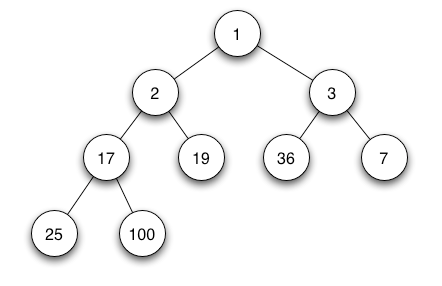
\includegraphics[width=1\linewidth]{figures/tree.png}
\caption{Min Heap Structure}
\label{fig:min_heap}
\end{figure}


\paragraph{Discussion}

The idea here is to use the min heap structure to obtain in a complexity of maximum $O(log(n))$  the point with the lowest priority. In the side we use a index map in order to replace point in the heap in an efficient way. Due to the fact that the design include the set of an element when it is already in the array. This structure has the advantage to benefit from static memory. The set works using the mapping to see if the point is already present in the map. If it is we replace it in the heap by changing his priority and apply a check with his ancestor then his descendant. If the point is not present we add a value at the end of the heap and check and update their ancestor to satisfy the condition of a min heap. So at the end the two operations needed for the algorithm reach a complexity of $O(log(n))$

\section{Postgres Implementation}

In this section we describe how the algorithm is implemented into the mobilityDB sql functions.
\subsection{SQL Code}

\begin{lstlisting}[
language=SQL, % Setting the language for SQL
caption={SQUISHE SQL Code}, % Caption for the listing
label=lst:squish_sql, % Label for referencing the listing
basicstyle=\ttfamily\small, % Basic style
keywordstyle=\color{blue}\ttfamily, % Style for keywords
stringstyle=\color{red}\ttfamily, % Style for strings
commentstyle=\color{green}\ttfamily, % Style for comments
numbers=left, % Line numbers on the left
numberstyle=\tiny\color{gray}, % Style for line numbers
stepnumber=1, % Line numbers step
frame=single,
breaklines=true, % Automatic line breaking
postbreak=\mbox{\textcolor{red}{$\hookrightarrow$}\space}, % Arrow for line breaks
showstringspaces=false % Don't show special spaces within strings
]
CREATE FUNCTION SquishESimplify(tfloat, float, boolean DEFAULT TRUE)
RETURNS tfloat
AS 'MODULE_PATHNAME', 'Temporal_simplify_sqe'
LANGUAGE C IMMUTABLE STRICT PARALLEL SAFE;
CREATE FUNCTION SquishESimplify(tgeompoint, float, boolean DEFAULT TRUE)
RETURNS tgeompoint
AS 'MODULE_PATHNAME', 'Temporal_simplify_sqe'
LANGUAGE C IMMUTABLE STRICT PARALLEL SAFE;
\end{lstlisting}

\subsection{Example}
This section show some examples of usages of the pgsql function describe in \ref{lst:squish_sql}. This allowed to use the algorithm in an offline settings using request.
\begin{lstlisting}[
language=SQL, % Setting the language for SQL
caption={Example SQL Code}, % Caption for the listing
label=lst:example_sql, % Label for referencing the listing
basicstyle=\ttfamily\small, % Basic style
keywordstyle=\color{blue}\ttfamily, % Style for keywords
stringstyle=\color{red}\ttfamily, % Style for strings
commentstyle=\color{green}\ttfamily, % Style for comments
numbers=left, % Line numbers on the left
numberstyle=\tiny\color{gray}, % Style for line numbers
stepnumber=1, % Line numbers step
frame=single,
breaklines=true, % Automatic line breaking
postbreak=\mbox{\textcolor{red}{$\hookrightarrow$}\space}, % Arrow for line breaks
showstringspaces=false % Don't show special spaces within strings
]

SELECT SquishESimplify(tfloat '[1@2000-01-01, 2@2000-01-02, 3@2000-01-04,
4@2000-01-05]', '1 day');
-- [1@2000-01-01, 3@2000-01-04]

SELECT asText(SquishESimplify(tgeompoint '[Point(1 1 1)@2000-01-01,
Point(2 2 2)@2000-01-02, Point(3 3 3)@2000-01-04, Point(5 5 5)@2000-01-05)', 0.5));
-- [POINT Z (1 1 1)@2000-01-01, POINT Z (3 3 3)@2000-01-04,POINT Z (5 5 5)@2000-01-05)

\end{lstlisting}

\subsection{Result}

Here we will talk about the result of the function and see the precision and the performance of the requests. We will also compare it with the C implementation in real time using the same data to compare the offline implementation with the online one.

\subsection{Performance}
This section will analyze and discuss the performance of the sql function by varying the lambda parameter and the number of points.
\begin{table}[htbp]
\centering
\label{tab:execution_time}
\begin{tabular}{@{}lccccc@{}}
\toprule
Number of Points & \multicolumn{5}{c}{Lambda} \\
\cmidrule{2-6}
& 1         & 0.75       & 0.5        & 0.25       & 0.01       \\
\midrule
100              & 00.001137 & 00.001965 & 00.002775 & 00.003328 & 00.004529 \\
1000             & 00.01498  & 00.014966 & 00.022183 & 00.024588 & 00.023035 \\
10000            & 00.164196 & 00.215692 & 00.214011 & 00.247379 & 00.218447 \\
100000           & 01.77365  & 02.171435 & 02.844324 & 02.617976 & 02.437037 \\
1000000          & 04.618455 & 05.371317 & 06.461961 & 06.021071 & 04.510934 \\
\bottomrule
\end{tabular}
\caption{Average Execution Time by Number of Points and Lambda}
\end{table}

In order to get those results we benchmark the request 10 times for each requests and retrieve the average of those executions. As standalone results it has no real meaning outside but we can notice that the speed of the algorithm increase around $0.5$ and decrease outside those values of lambda. We can also state that maybe there is another value as maximum execution time between $0.75$ and $0.25$ . We can state that this is maybe because the number of instruction that mix setting in a priority queue and the instructions of reduction is around $0.5$. Because when lambda is equal to 1 there is no reduction and only setting in the maximal size of a priority queue and adjust priority operation and when lambda go towards $0$ there is a lot of reduction operation and setting in the minimal size of a priority queue. That is an explanation that could befit those data. When the size of the input is multiplying by $10$ the execution time is around $2$ times longer.

\paragraph{Comparison with C}
In order to have meaning to those result we will compare it with the C implementation using the real time approach and to see between the offline and the online approach the difference that happen.

\begin{table}[htbp]
\centering
\label{tab:execution_time_c}
\begin{tabular}{@{}lccccc@{}}
\toprule
Number of Points & \multicolumn{5}{c}{Lambda} \\
\cmidrule{2-6}
& 1         & 0.75       & 0.5        & 0.25       & 0.01       \\
\midrule
100              & 00.000094 & 00.000092 & 00.00009 & 00.000098 & 00.000096 \\
1000             & 00.00081  & 00.000822 & 00.000943 & 00.000876 & 00.000788 \\
10000            & 00.008889 & 00.008852 & 00.008663 & 00.008263 & 00.00818 \\
100000           & 00.090018  & 00.088485 & 00.089533 & 00.089064 & 00.088728 \\
1000000          & 00.892172 & 00.864116 & 00.870661 & 00.937186 & 00.920517 \\
\bottomrule
\end{tabular}
\caption{Average Execution Time (C) by Number of Points and Lambda}
\end{table}

As we can see, executing C code is much faster than executing sql queries, which makes execution and simplification using steam processing techniques in C both viable and possible. The speed is such that even for 1 million points the average execution time is less than 1 second.

\subsection{Precision}
This section will focus on the precision of the simplification using the same parameter as before in order to have an idea of the quality of the simplification in a function of lambda and types of path. We will discuss on trajectory based on AIS dataset. As stated in \cite{abam2007streaming}, there is different type of path as convex and concave. As a reminder this work focus on the simplification of lines and do not take into account land or see restriction during the simplification process. In this section we will analyze different trajectory defines them and see with different lambda and metrics evaluation the quality of the simplification. At the end we will run in a big datasets and see the results as a graph and discuss them.

\paragraph{Trajectory 1}

\begin{figure}[!h]
\centering
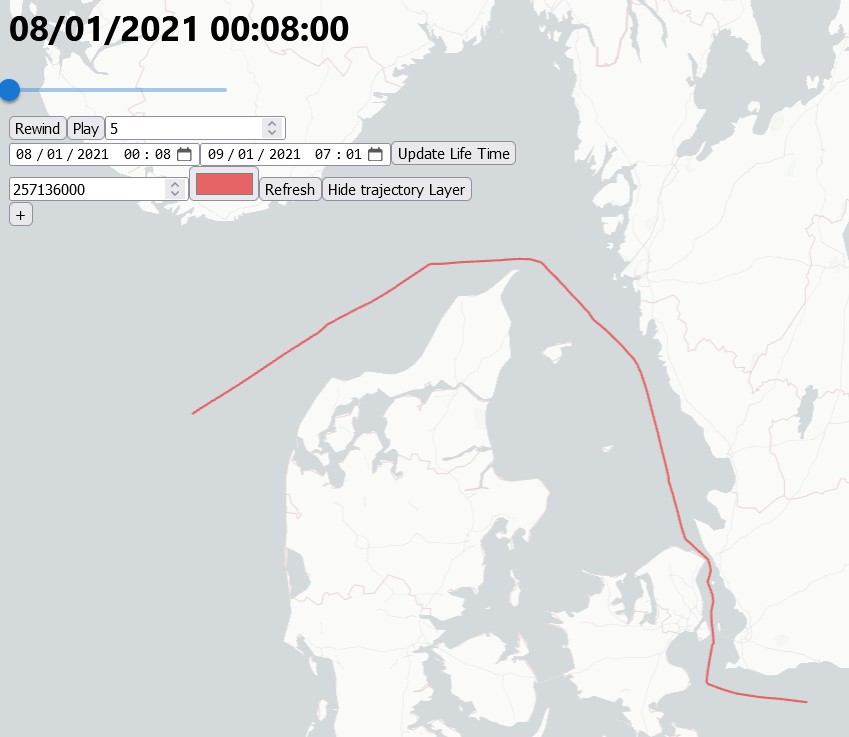
\includegraphics[width=0.5\linewidth]{figures/Stats/traj_1.jpg}
\caption{Trajectory 1}
\label{fig:traj_1}
\end{figure}

This trajectory is composed of 20865 points and begin at 1am the 8/1/2021 with a duration of 1 day. This trajectory have convex and concave path in order to analyze the effect of the simplification in those specific moment. The precision of the trajectory will be computed based on the current metrics proposed in the state of the art such as frechet distance and hausdorff distances. We will not discuss the precision of lambda 1 because it does not reduce any points from the original trajectory.



\begin{figure}[!h]
\centering
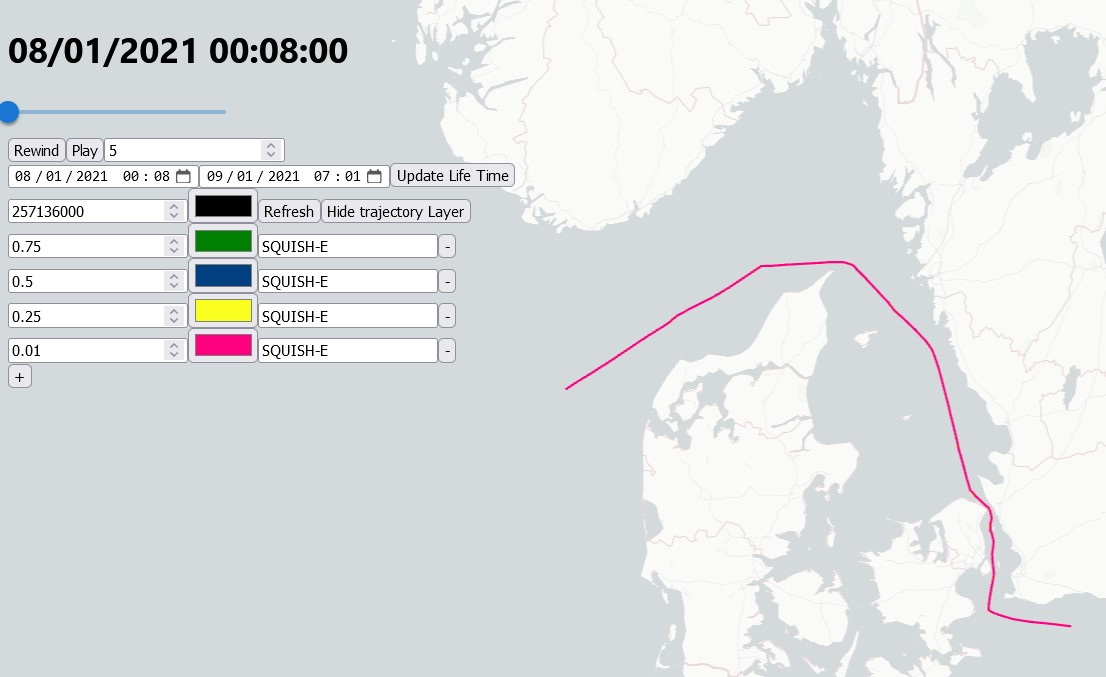
\includegraphics[width=0.5\linewidth]{figures/Stats/squish_1.jpg}
\caption{Trajectory 1 - SQUISH-E}
\label{fig:traj_1_squish}
\end{figure}

The path looks really similar and is close to the original path in \ref{fig:traj_1_squish}. In order to see the differences we can zoom and move the slider in order to see the moving objects in relation with the current time.

\begin{figure}[!h]
\centering
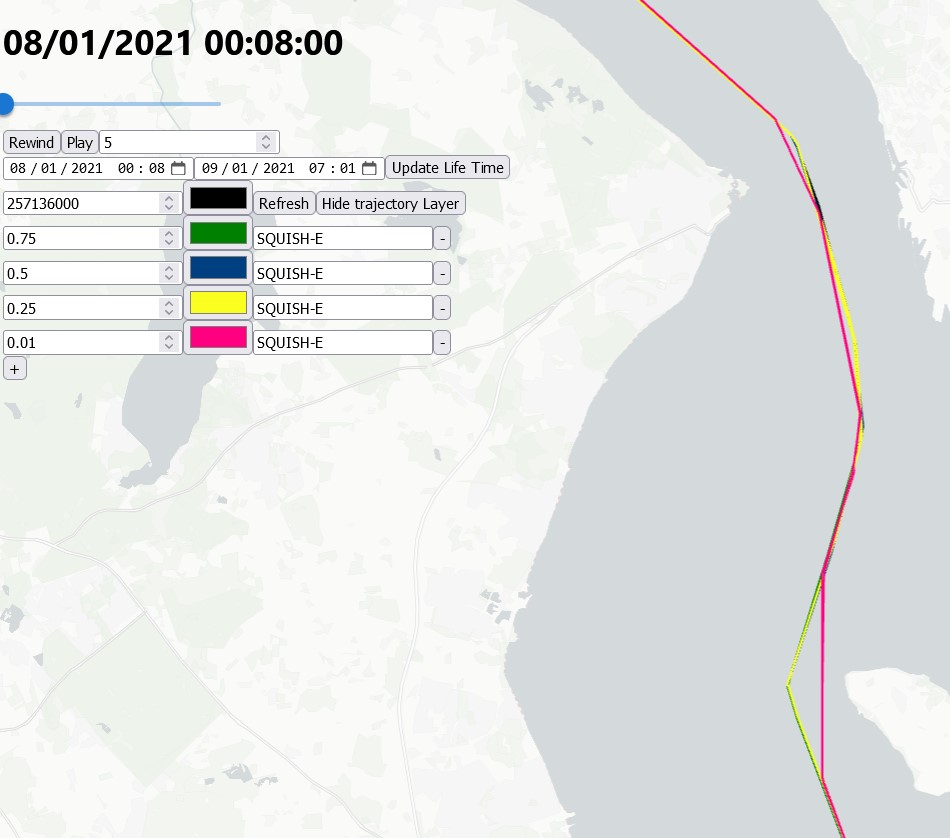
\includegraphics[width=0.5\linewidth]{figures/Stats/squish_1_zoom.jpg}
\caption{Trajectory 1 - ZOOM }
\label{fig:traj_1_sqzoom}
\end{figure}

In this we can see the path being simplified where there is curves and having less precision as lambda decreases.

\begin{table}[htbp]
\centering
\label{tab:precision_metrics}
\begin{tabular}{@{}lcccc@{}}
\toprule
& \multicolumn{4}{c}{Lambda} \\
\cmidrule{2-5}
& 0.75       & 0.5        & 0.25       & 0.01       \\
\midrule
Number of points           & 15648 & 10432 & 5215 & 208 \\
Frechet Distance              & 818.006 & 818.006 & 818.006 & 6902.445 \\
Hausdorff Distance             & 818.006 & 818.006 & 818.006 & 6902.445 \\
DynTimeWarp Distance            & 80452.262 &  236389.238 & 634626.475 & 22557588.744\\
Temporal Distance            & 0.909 & 1.712 & 2.635 & 49.748\\
\bottomrule
\end{tabular}
\caption{Precision metrics per Lambda for Trajectory 1 }
\end{table}

This table gives a view of the precision of squish-e on the first trajectory. The data shows that it is consistent and precise and that errors is increasing when lambda decreases. Dynamic Time Warping Distance gives also an overview of the loss of precision when we remove more points.

\paragraph{Comparison With C}
This section will outline the differences between the SQL and C execution since the SQL represents an offline execution and C represents the online the differences here is to underline the possible loss of accuracy in the process. In order to keep this part concise a table with all variables above will be given and choose the differences of the distances between the offline and the online trajectories.

\paragraph{Trajectory 1}

\begin{table}[htbp]
\centering
\label{tab:precision_metrics_c}
\begin{tabular}{@{}lcccc@{}}
\toprule
& \multicolumn{4}{c}{Lambda} \\
\cmidrule{2-5}
& 0.75       & 0.5        & 0.25       & 0.01       \\
\midrule
Difference of points           & 208 & 254 & 154 & 7 \\
Difference of Frechet Distance              & 0 & 0 & 0 & -393.393 \\
Difference of Hausdorff Distance             & 0 & 0 & 0 & -393.393 \\
Difference of DynTimeWarp Distance            & 555.155 & 6945.389 & 22660.099 & 830547.714\\
Difference of Temporal Distance            & 0.0284 & 0.0239 & 0.0175 & 1.842\\
\bottomrule
\end{tabular}
\caption{Comparison Precision metrics per Lambda for Trajectory 1 }
\end{table}

The comparison shows that the offline and online implementations provide different numbers of trajectory points. Because of its gradual processing, we find that the online version typically produces more points, while the offline version might use more forceful compression methods.

We examine the success of both offline and online implementations using metrics for trajectory similarity. For smaller lambda values, the two solutions perform similarly on average; however, differences appear when the compression level is increased. In particular, because of its comprehensive approach to trajectory analysis, the offline implementation might yield similarity metrics that are more accurate.

Lets additionally look at the temporal properties of the paths that the two implementations process. Our investigation reveals possible variations in temporal synchronization and alignment, with consequences for applications needing accurate temporal matching.

The offline version shines in accuracy and thorough analysis, while the online version offers real-time processing capabilities and adaptability to dynamic data streams. The selection between the two paradigms is contingent upon particular application needs, such as the demand for accuracy, real-time responsiveness, and resource restrictions.




